\begin{figure}[t]
\centering
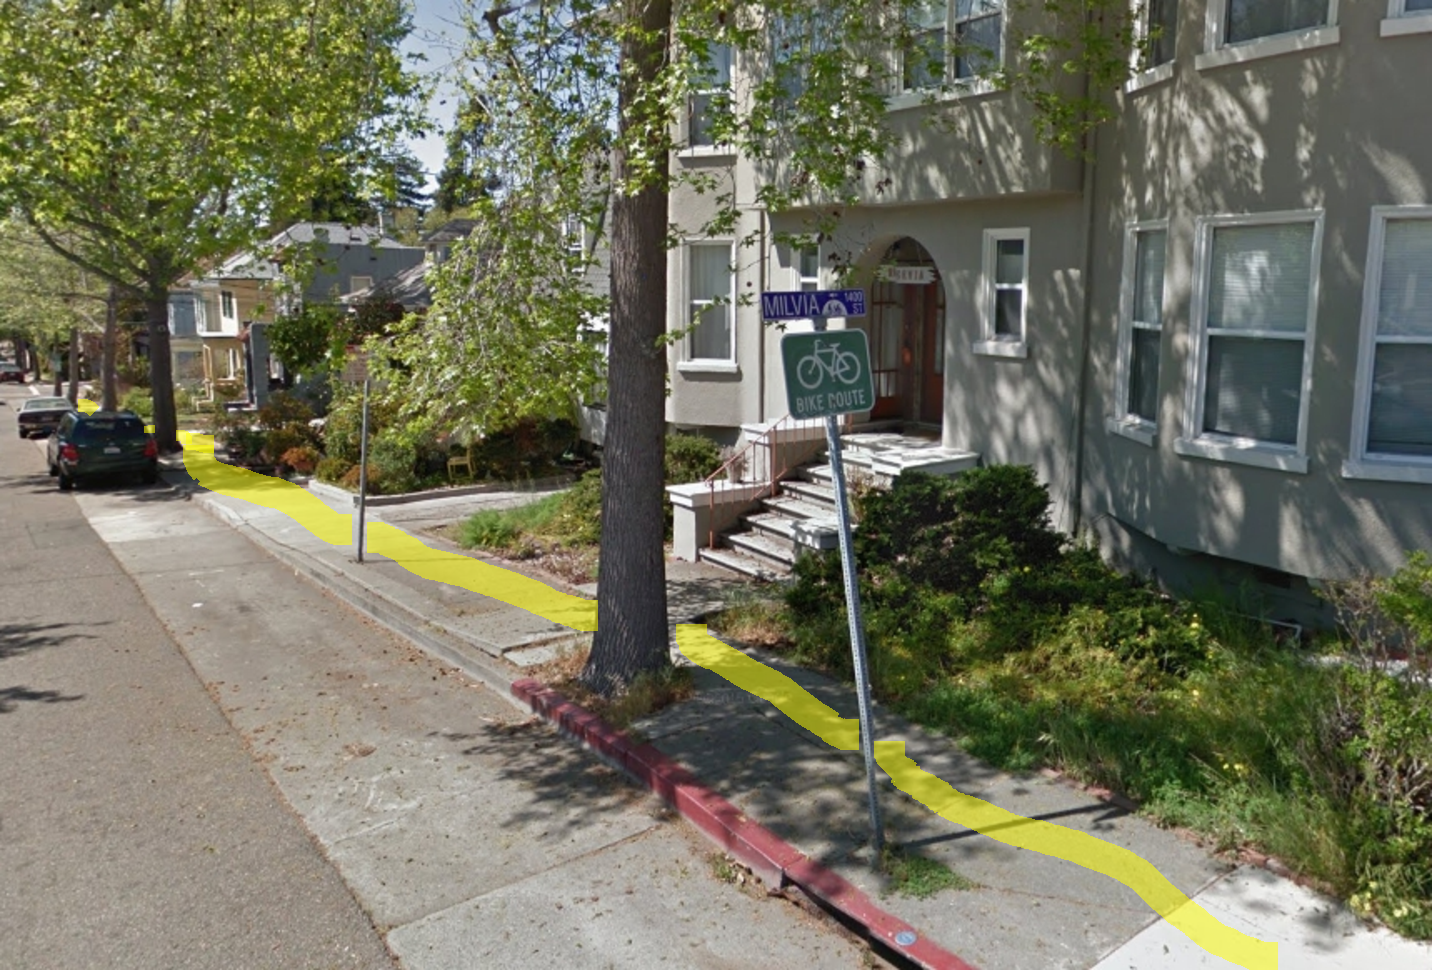
\includegraphics[width=\linewidth,,trim=0 0 0 0,clip]{paper/content/images/evaluation_path}
\caption{Segment of Evaluation Circuit}
\label{fig:evalpath}
\end{figure}

\section{CONCLUSION \& FUTURE WORKS}
\label{sec:conclusion}
This paper proposes a methodology for training DNNs to perform in several distinct behavioral modalities simultaneously, through the insertion of modal information. This MultiNet approach is shown to exceed the performance of multiple individual networks trained separately, while using fewer parameters. The MultiNet networks are shown to be more resistant to overfitting as well as capable of developing more specific behaviors characteristic of the behavioral mode of operation. These results are verified with real world evaluation of the networks in sidewalk driving situations using 1/10th scale model cars. Future work could include work on adapting the approach to full size vehicles as well as implementation of MultiNet architectures in other type of neural network models, such as recurrent networks. Additionally, in the future work could be done to make modal information available from higher-level networks trained to select behavioral modes, thereby granting the system a qualitatively higher level of autonomy.
